\section{List}

I dette afsnit vil arkitekturen for widgettypen List blive præsenteret. Dette vil ligge grundlag for at en uddybende beskrivelse af hvordan widget'en er designet og implementeret.

List har været under udvikling næsten hele semestret, hvor sidste prik over i'et blev sat under 6. iteration. Udviklingen af List kan afspejles i nedenstående figur, der viser hvilket funktionaliteter List har fået under forskellige iterationer.

\begin{figure}[H]
    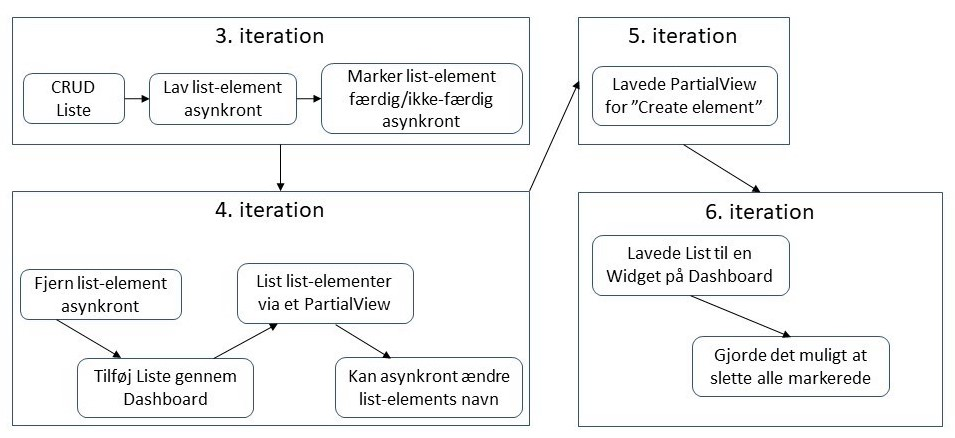
\includegraphics[width=\linewidth]{09_Arkitektur/Lists/Images/Iterationer.jpg}
    \caption{Figuren viser hvordan List har været under udvikling i lang til. Dette afspejler meget at udviklingen har givet mere viden undervejs, hvilket har ledt til optimering.}
    \label{fig:ListIterationer}
\end{figure}

I den sidste iteration blev der også gjort sådan at ListItems bliver streget ud gennem JavaScript inden der modtages et nyt PartialView fra serveren.

\subsection{Data view}

Relationen mellem en liste og dens list-elementer er en-til-mange, da en liste skal kunne have mange ListItems. En ListItem har en composite key, som består af ListId og ListItemId, hvilket giver en god dataintegritet, sådan at de ListItems der bliver vist rent faktisk tilhører den samme liste.

\begin{figure}[H]
    \centering
    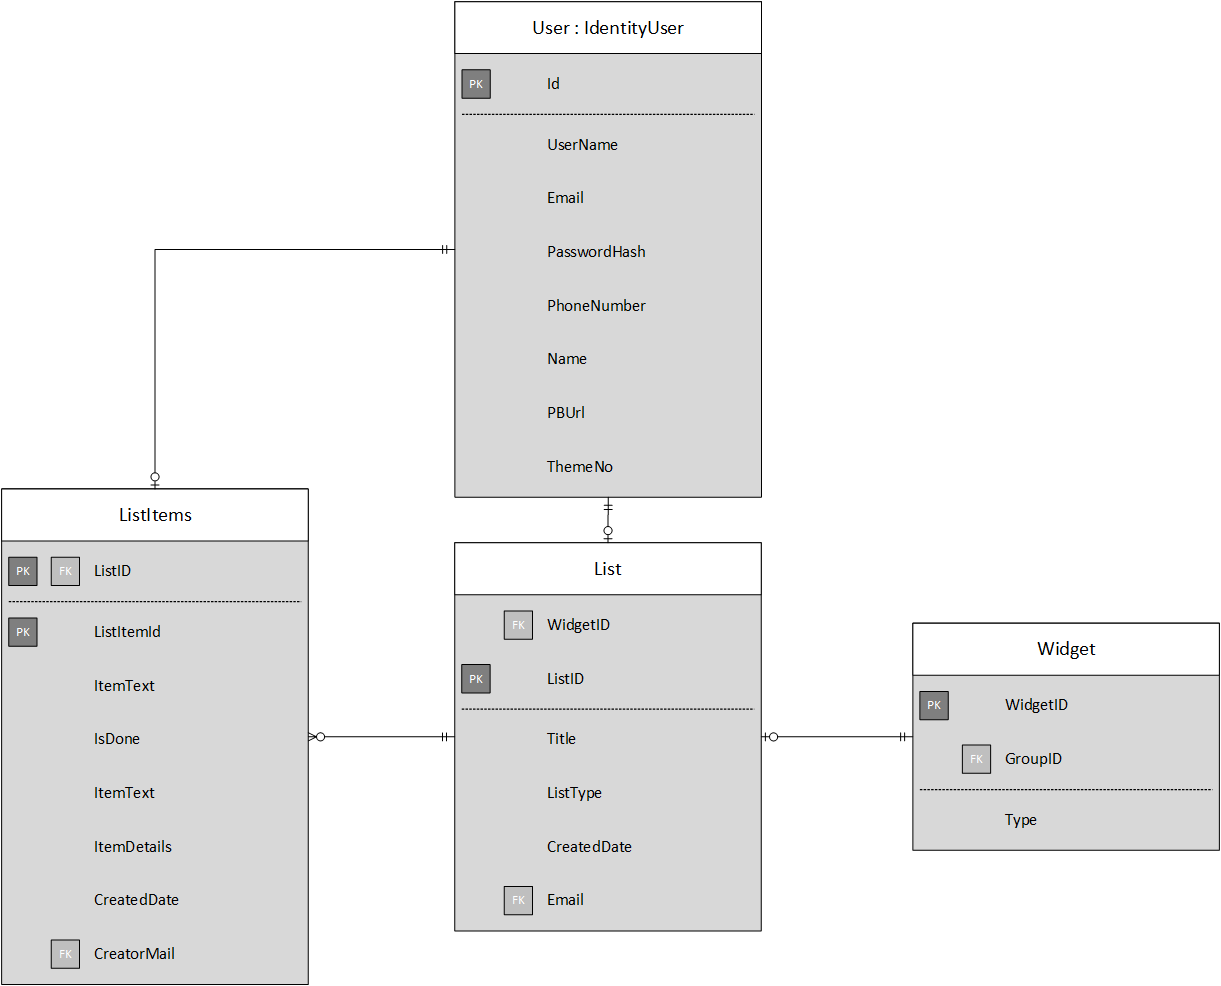
\includegraphics[width=0.9\linewidth]{09_Arkitektur/Lists/Images/ListDbFinal.png}
    \caption{Da List har været under udvikling i mange iterationer, har dataen for List også ændret sig. Bl.a. ListType og CreatorMail er noget der er blevet tilføjet løbende.}
    \label{fig:ListDbFinal}
\end{figure}

CreatorMail for en ListItem er specielt hensigtsmæssig, så man kan se hvem der har lavet list elementet. 

\subsection{Logical view}

List har forholdsvis mange funktionaliteter gemt i sig. En widget har ikke meget plads på dashboard, og det er derfor begrænset hvad der kan være i den lille boks. Selvom det er gjort muligt at udvide boksende, er det dog stadig at foretrække at alt kan ses direkte, i stedet for at skulle folde den ud. På nedestående figur ses arkitektur for hvordan alle funktionaliteterne er wrappet sammen ud fra én fokuseret liste.

\begin{figure}[H]
    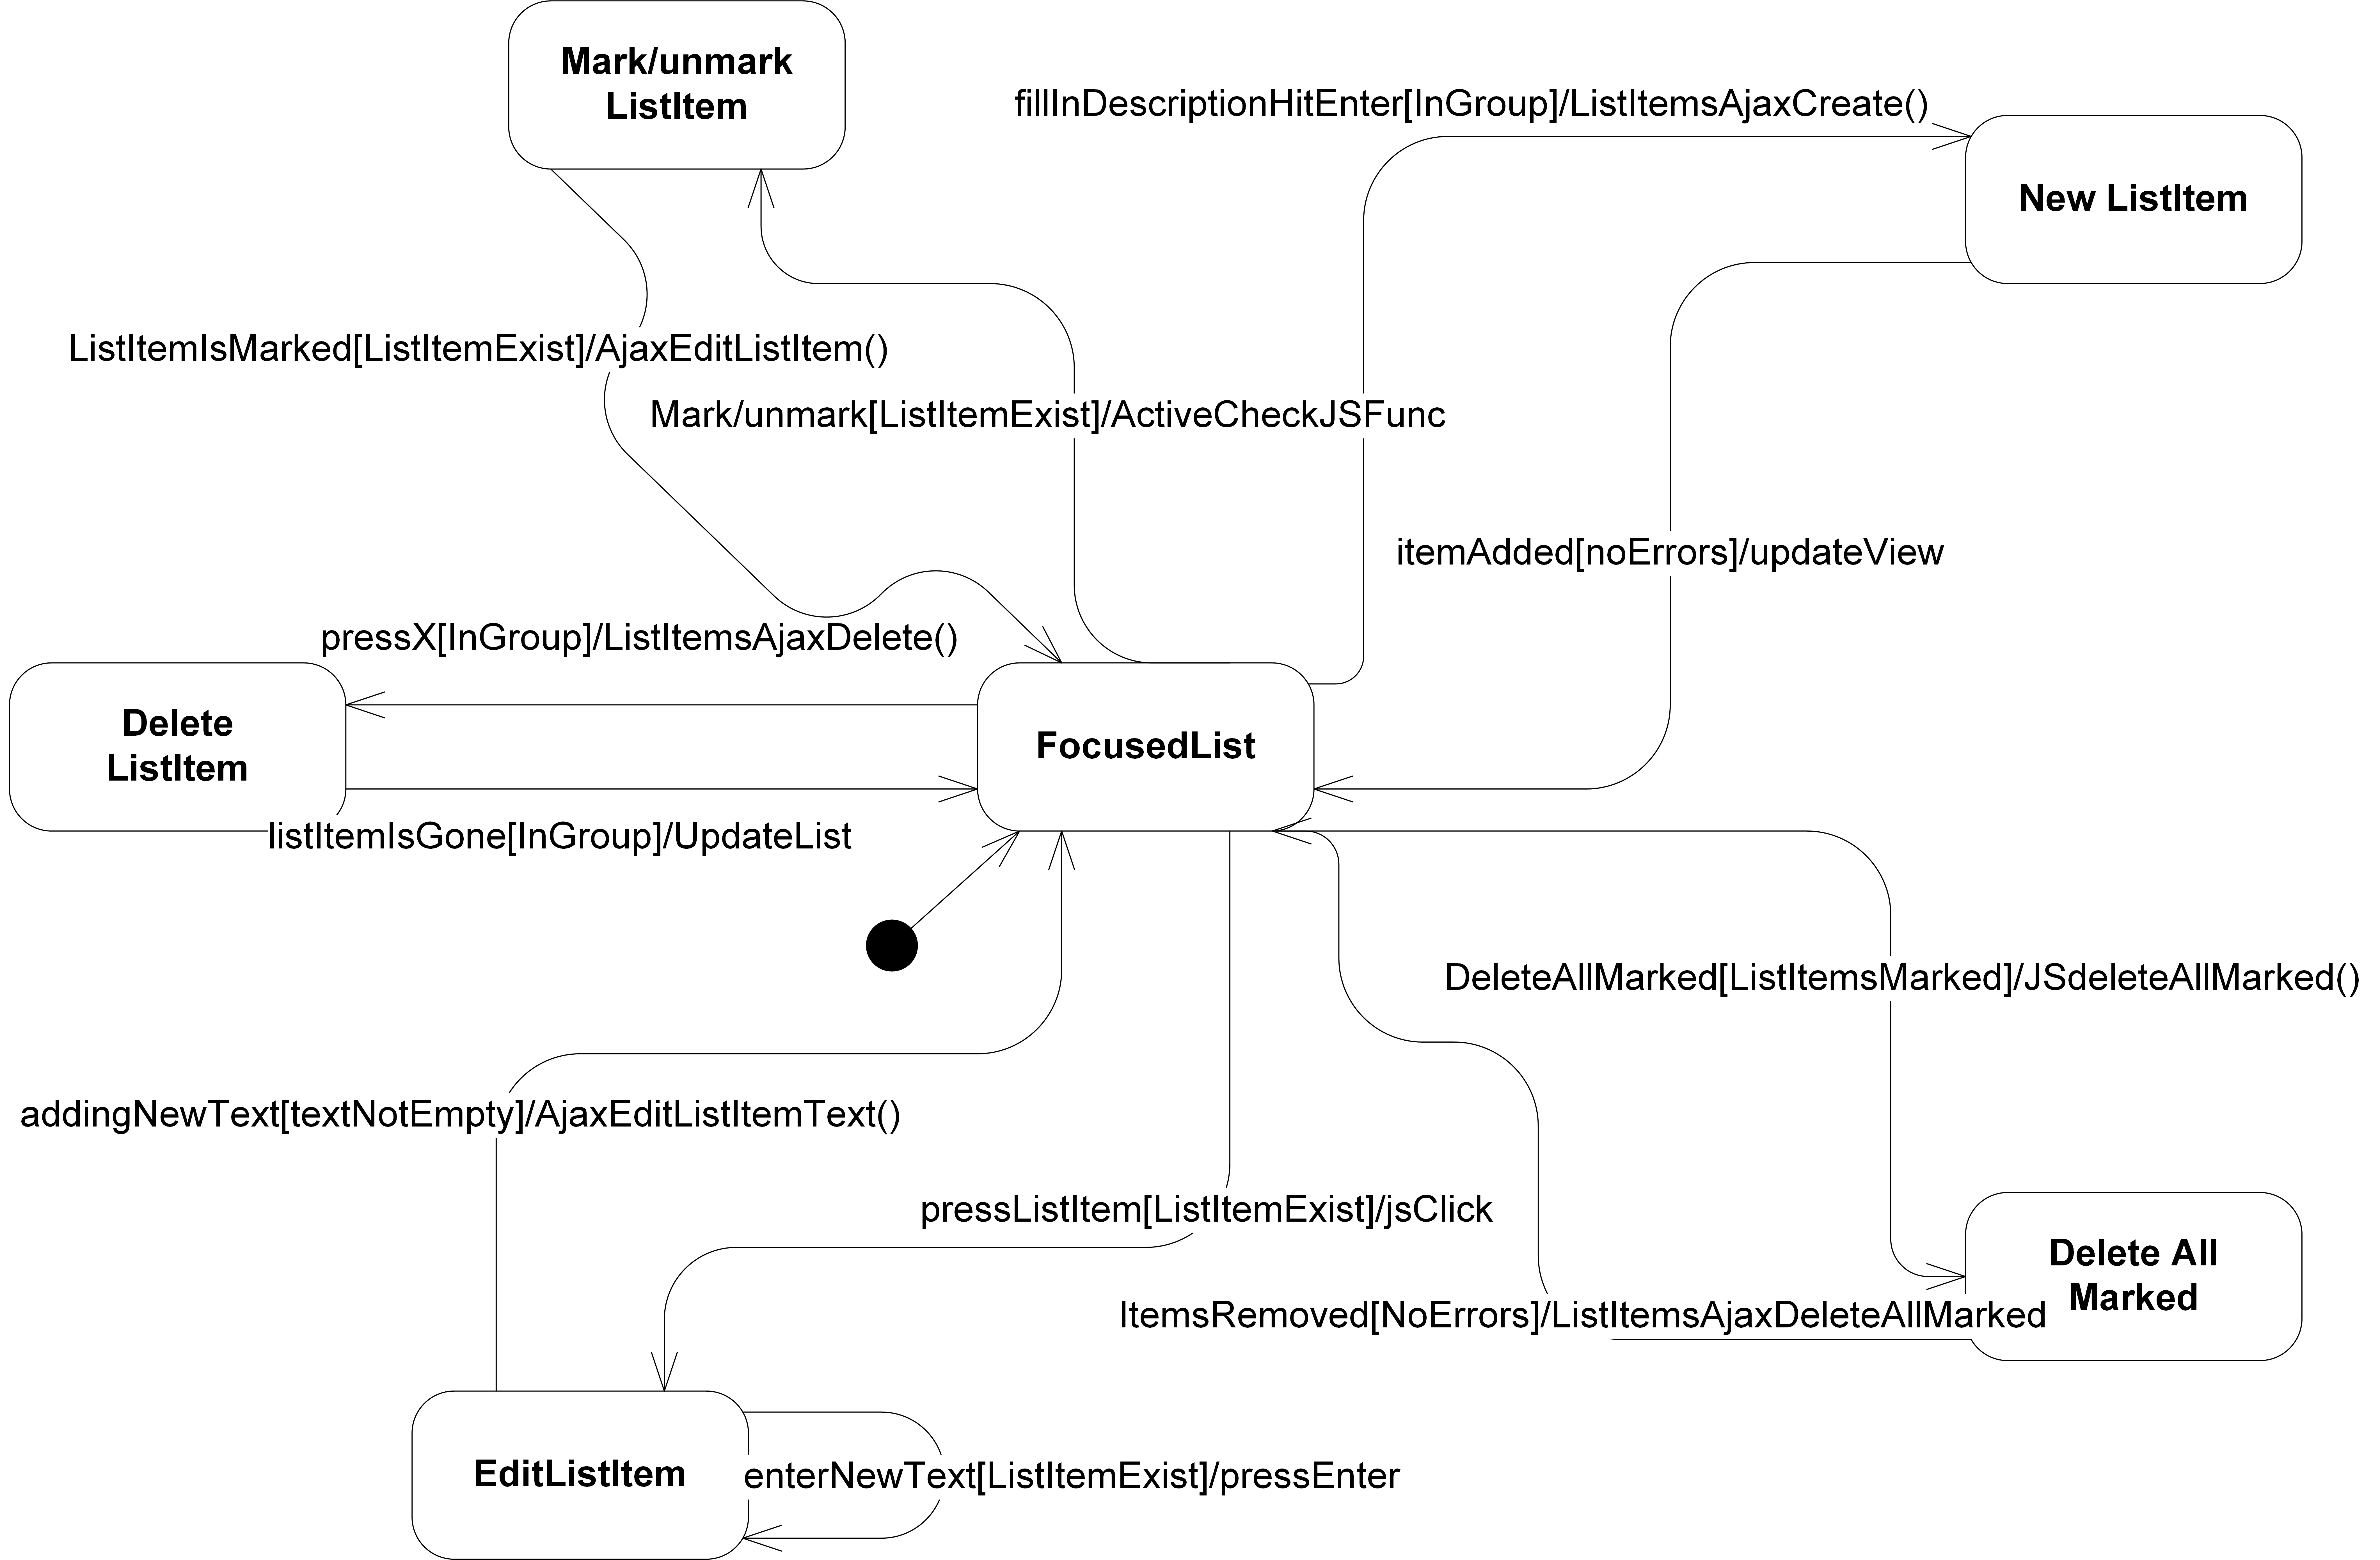
\includegraphics[width=\linewidth]{09_Arkitektur/Lists/Images/List_SM.png}
    \caption{Denne state machine viser hvilke funktionaliteter der er mulige at gøre med en widget af typen List. Dog er det valgt kun at gøre det muligt for skaberen af listen, at bruge funktionen med Delete All Marked. Dette kan dog nemt laves om, men blev bedømt til at være være lidt risikofyldt ellers.}
    \label{fig:list_stm}
\end{figure}

I bilagende er der lavet sekvensdiagrammer der demonstrerer disse funktionaliteter, hvor nogle er udeladt, da sekvenserne bliver meget ensformige. I stedet for at Delete All Marked kun kan gøres af ejer, kunne det evt ændres til at alle kan gøre det, men at de bliver spurgt om de er sikre på deres valg.